% template

\documentclass[a4paper,12pt,titlepage]{article}

\usepackage{CJKutf8}
\usepackage{amsmath}
\usepackage{indentfirst}
\usepackage{float}
\usepackage{graphicx}
\usepackage{longtable}

\setlength{\parindent}{2em} 

\begin{CJK*}{UTF8}{gbsn}
\begin{document}

\title{图形学大作业-模拟银河系}
\author{物理学院\ 秦光辉\ 曾嘉熙}
\maketitle

\tableofcontents
\newpage

\section{程序环境}

\subsection{Windows}

	在 Windows 10 中可以直接运行可执行文件. 编译环境为 VS 2017, 32 位编译. 需要外部依赖库:
	
\begin{itemize}
	\item GLEW
	\item GLFW
	\item GLM
\end{itemize}

	这些依赖库我们已经在文件夹 external 中提供, 默认版本为 32 位版本. 如果需要 64 位版本, 则需要自己添加或者编译. \\
	
	程序运行需要 22 个 DDS 文件(编号从0到20, 外加一个字体包). 需要一个 GLEW 的 DLL 动态链接库, 需要 5 个 obj 模型文件, 需要一个 bmp 贴图. 文件夹中有四个我们所写的 shader 文件, 也需要加在运行目录下.

\subsection{Ubuntu}

	在 Linux 环境下可以直接编译, 前提是系统中有上述三个依赖库. 在 ubuntu 下使用 qt ide 可以正常编译运行.

\section{程序模块}

\subsection{模拟银河系介绍}

	银河系中有几千亿颗恒星, 辽阔宽广. 我们希望不仅能够模拟出单个的恒星和它所拥有的行星系统, 而且能够把整个银河系几千亿颗恒星都能够独一无二的表现出来. 独一无二不仅是每一颗恒星都是不一样的, 而且要求每次到达这个区域(不论中途进行了什么操作), 这颗恒星(包括所拥有的行星系统)都存在于这个区域中. \\
	
	但是上千亿颗恒星过于复杂, 远远超出计算机的处理能力. 所以需要合理的随机算法和合理的显示手段. 同时作为物理学院的学生, 我们不能做出一个不合理的银河系来. 在宇宙中穿梭, 即使有再强大的动力, 也不可能超过光速. 同时相对论效应将会不可避免的被计入在内. 我们的程序做了最大努力, 希望能够还原出真实的狭义相对论效果, 包括物理的形变, 位移, 红移, 蓝移和亮度变化等. \\
	
	下面我们将分模块介绍程序.
	
\subsection{随机函数}

	我们所处的银河系是柱状星系, 有两个悬臂, 在悬臂所处的范围内恒星密集, 在悬臂之外恒星稀疏. 我们希望能够模拟出真实的悬臂效果. 为此我们把整个宇宙模拟成一个 100000 * 100000 * 1000 大小的方盒(这个比例和真实银河系相同). 方盒内每一个空间里最多只有一颗恒星. 方盒内有一个密度函数, 表征每一个点的恒星密度. 这个函数的计算方式如下:
	
\begin{enumerate}
	\item 给定一个点的坐标
	\item 如果这个点在方盒外, 返回0
	\item 按照阿基米德螺旋线旋转这个点, 到达新的位置
	\item 计算这个点与 y 轴的距离, 得到 r
	\item 把r代入一个指数函数形式的非线性函数, 返回结果值
\end{enumerate}

	这个算法保证了空间中每个点都有一个密度值, 而且越靠近悬臂的地方密度越大, 在悬臂之外密度值低, 这样就可以得到一个合理的密度函数. \\
	
	然后我们使用了一种特殊的随机算法. 空间中每一个区域都有一个独一无二的坐标值, 把三个坐标值代入一个质数取模和求和运算中, 得到一个数值, 将该数值代入随机数种子中, 然后利用 C++ 的随机函数得到一个随机序列. 使用这个序列可以确定这个区域内是否有恒星存在, 如果存在, 进而确定这颗恒星的所有参数. 这些参数是和这个区域坐标绑定且独一无二的. \\
	
	这颗恒星的行星系统可以用类似的方法得到. 如果驾驶飞船远离恒星, 恒星会被系统从内存中清除, 但是如果再次回到这个空间位置, 同样的恒星和同样的行星会被加载出来(这是我们算法的特性).

\begin{figure}[H]
\centering
	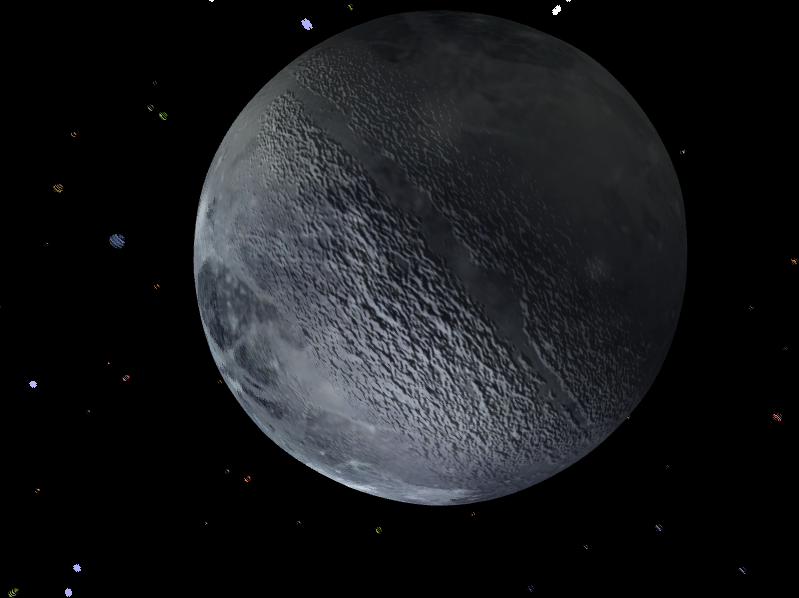
\includegraphics[scale=0.3]{03.png}
	\caption{近距离观察一颗行星(添加了bump map效果)}
\end{figure}
	
\begin{figure}[H]
\centering
	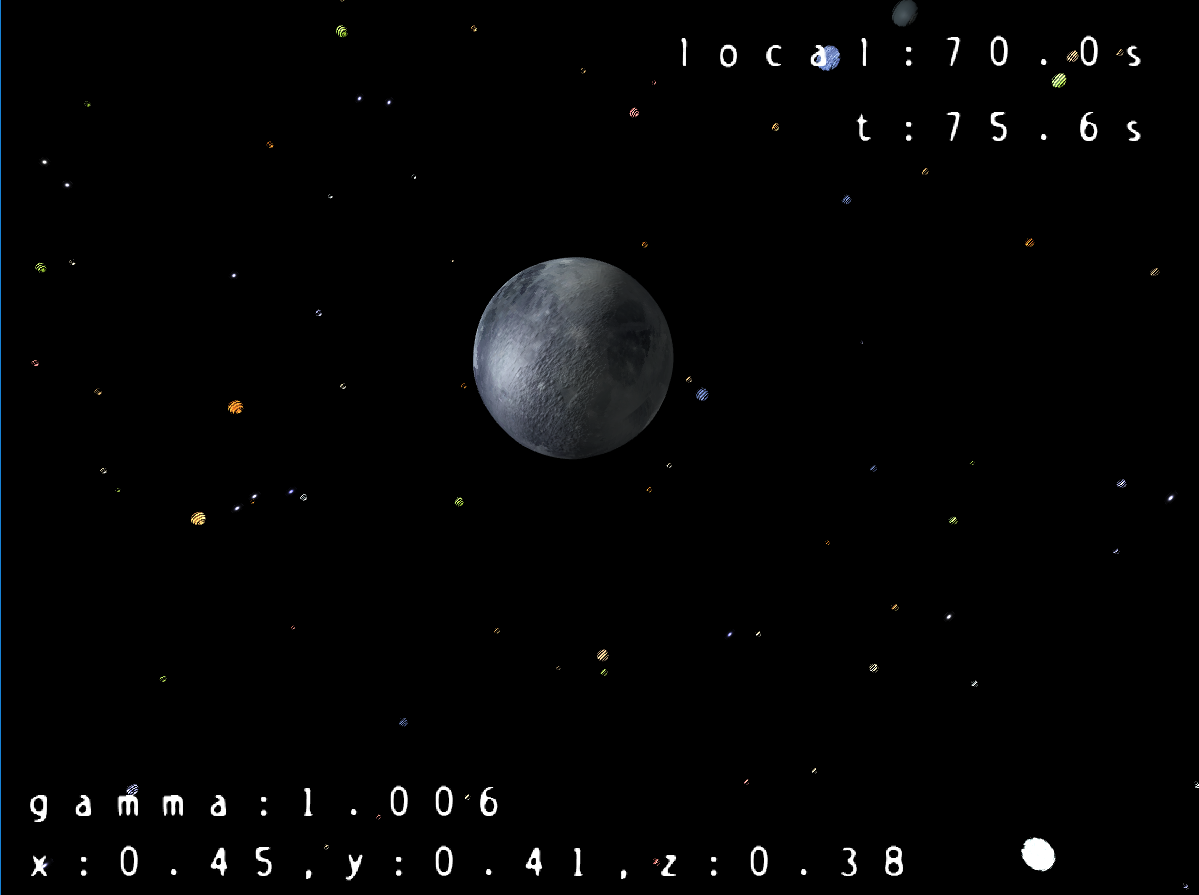
\includegraphics[scale=0.3]{04.png}
	\caption{远距离观察一颗行星(行星被恒星照亮)}
\end{figure}
	
\begin{figure}[H]
\centering
	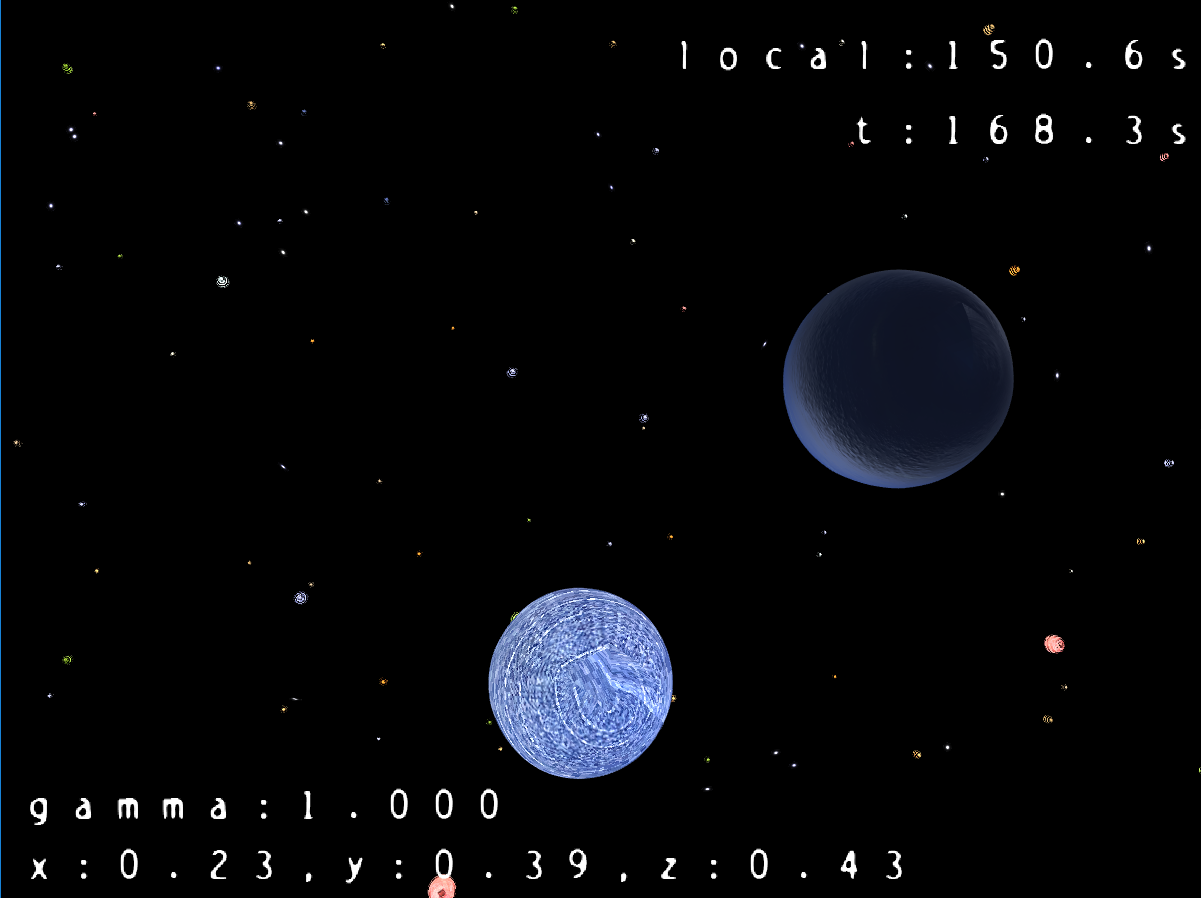
\includegraphics[scale=0.3]{05.png}
	\caption{绕着恒星转动的行星}
\end{figure}
	
\begin{figure}[H]
\centering
	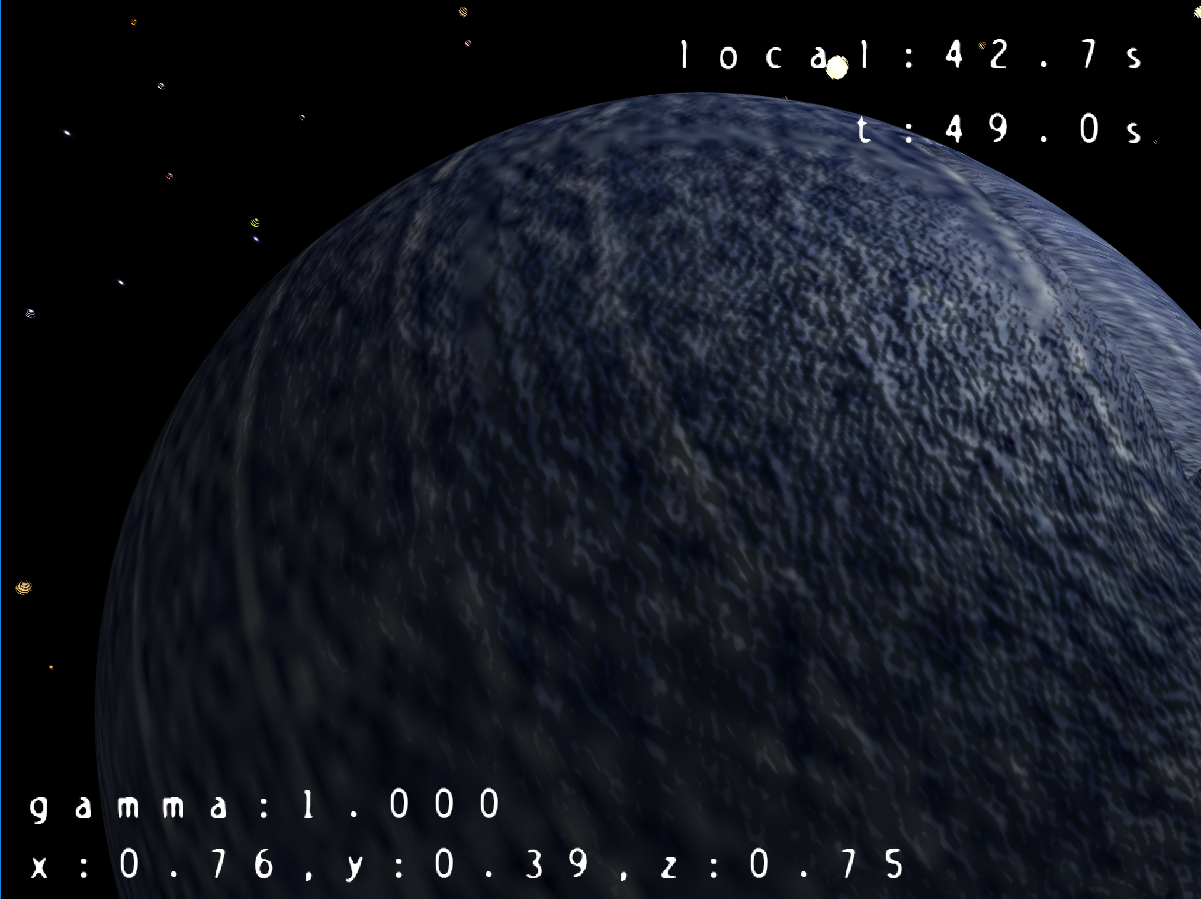
\includegraphics[scale=0.3]{06.png}
	\caption{行星的明暗分界线}
\end{figure}
	
\subsection{模型加载和 Monte Carlo 算法}

	飞船每次进入新的区域, 都会加载新的地图(这个加载是非常快的, 不会感觉到卡顿). 我们把整个空间分成四个区域. 首先是当前所处的 zone, 这个区域内的恒星会加载最精细的模型, 以达到最好的显示效果. 距离当前位置不远的恒星(具体来说是两格之内) 会加载第二档模型. 在较远距离会加载大约1000个区域的恒星, 这些恒星只会加载一个最粗糙的模型. \\
	
	但是如果只加载这些恒星, 宇宙会非常空旷. 如果恰好处于一个恒星稀疏的区域, 会看到整个宇宙都是黑暗的, 这是不合理的. 所以我们使用了 Monte Carlo 算法来加载上述区域之外的恒星. 算法会从当前位置发射若干条射线, 在射线上随机取点, 如果随机取点处恰好有恒星, 则在幕布上涂一个亮点. 否则保持黑暗. 最后把整个幕布加载到一个巨大的球体上, 作为贴图展示给玩家. 
	
\begin{figure}[H]
\centering
	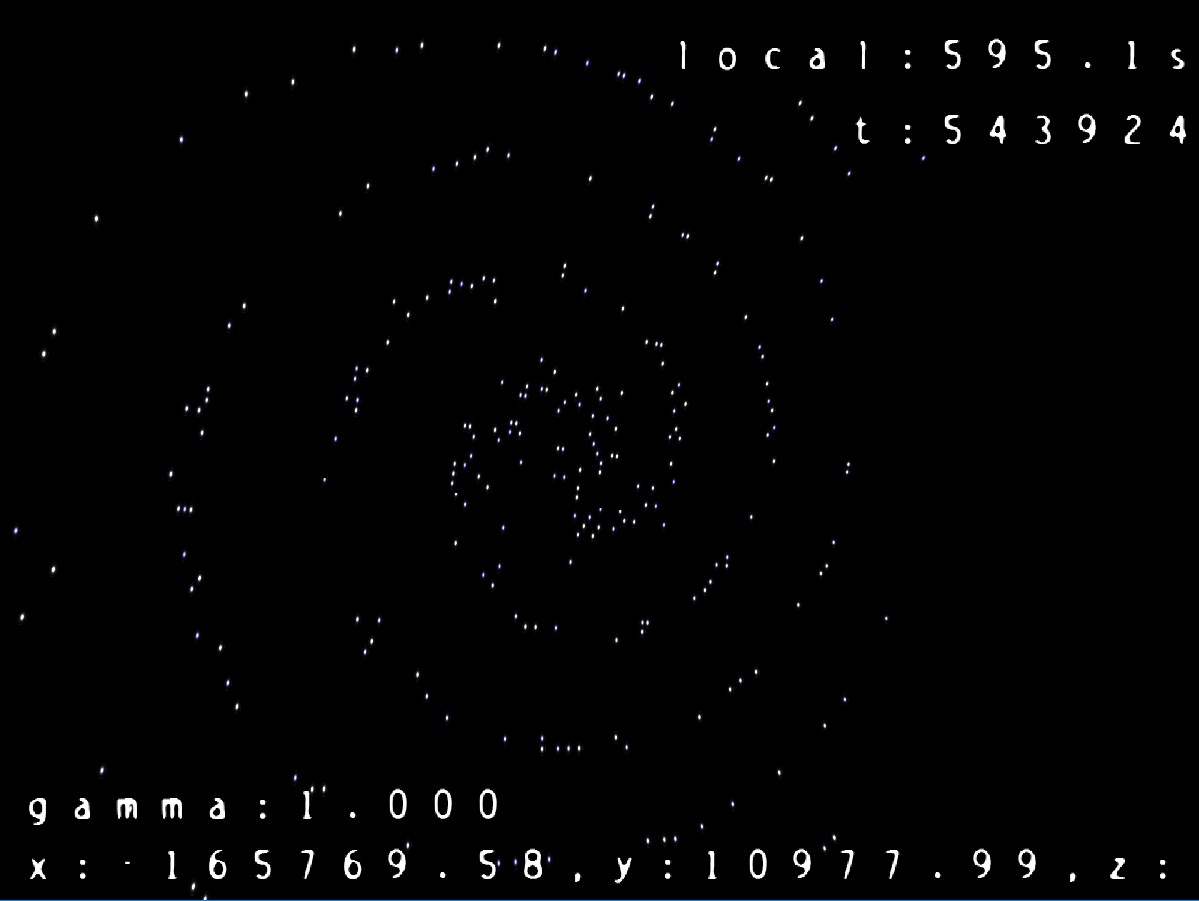
\includegraphics[scale=0.3]{00.png}
	\caption{从背后观察银河系, 使用了 Monte Carlo 进行贴图}
\end{figure}
	
\begin{figure}[H]
\centering
	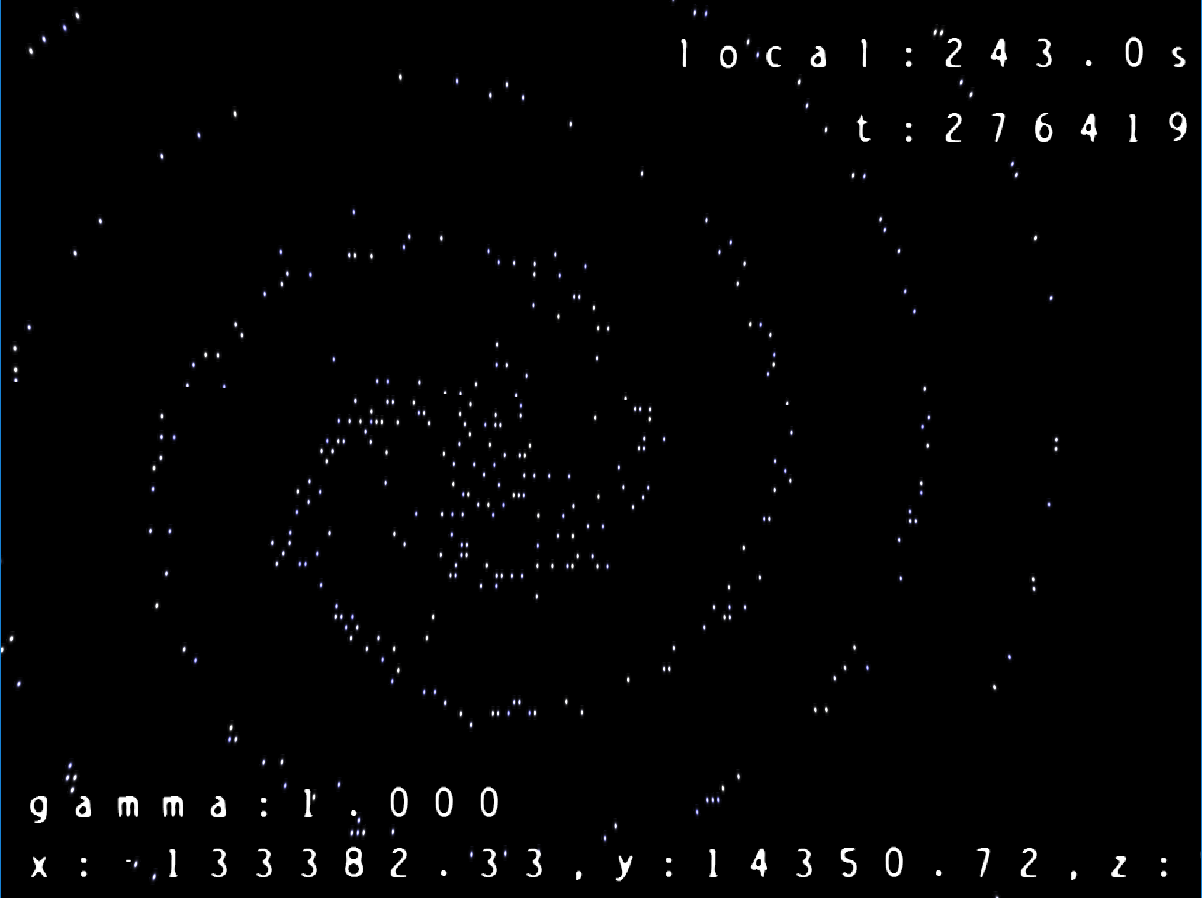
\includegraphics[scale=0.3]{01.png}
	\caption{从正面观察银河系}
\end{figure}
	
\begin{figure}[H]
\centering
	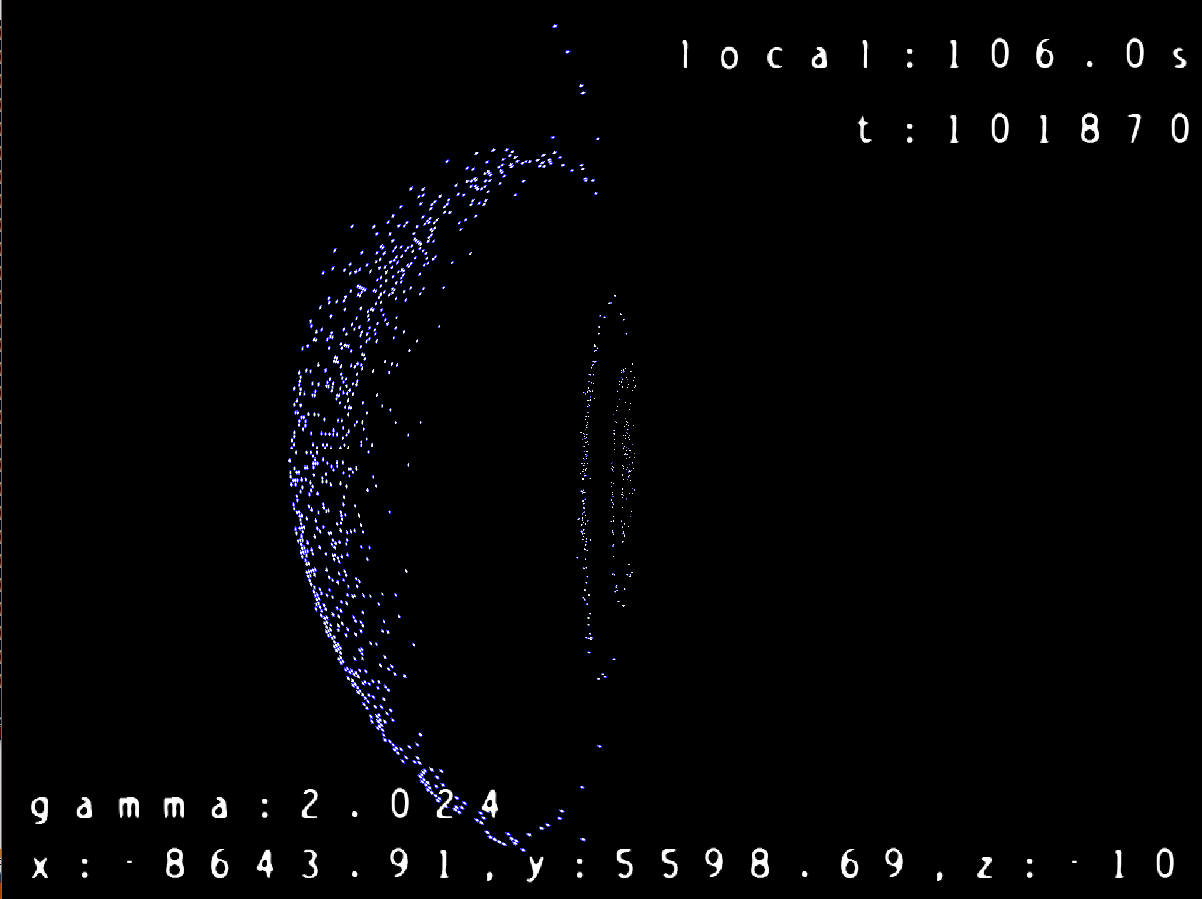
\includegraphics[scale=0.3]{02.png}
	\caption{从侧面观察银河系(加速的情况下的相对论修正)}
\end{figure}	

	行星表面有 bump map 贴图, 实现方式是加入bump map 贴图然后修改法向量. \\
	
	Monte Carlo 的贴图使用了特殊的 GLSL 的 shader 以避免贴图显示效果过差, 具体的修正在 shader 中有所体现. 此部分工作由曾嘉熙完成.
	
\subsection{相对论修正}

	作为物理学院的学生, 我们认为一个正确的宇宙模型渲染器必须包括相对论修正. 我们做了如下处理: \\
	
	在 myVertexShader.vertexshader 顶点渲染器中, 我们可以根据当前的速度值和运动方向, 使用 Lorentz Transform 对所有定点进行坐标变换, 产生形变和位移的视觉效果. \\
	
	在 myFragmentShader.fragmentshader 片段渲染器中, 我们使用 Lorentz Transform 计算每一个像素的 Doppler 效应因子, 进而计算每一个像素的颜色和亮度变化. \\
	
	具体的物理推导在此不赘述. 我们通过计算使其全部转换为矩阵运算, 以使得它可以在 GPU 中计算.

\begin{figure}[H]
\centering
	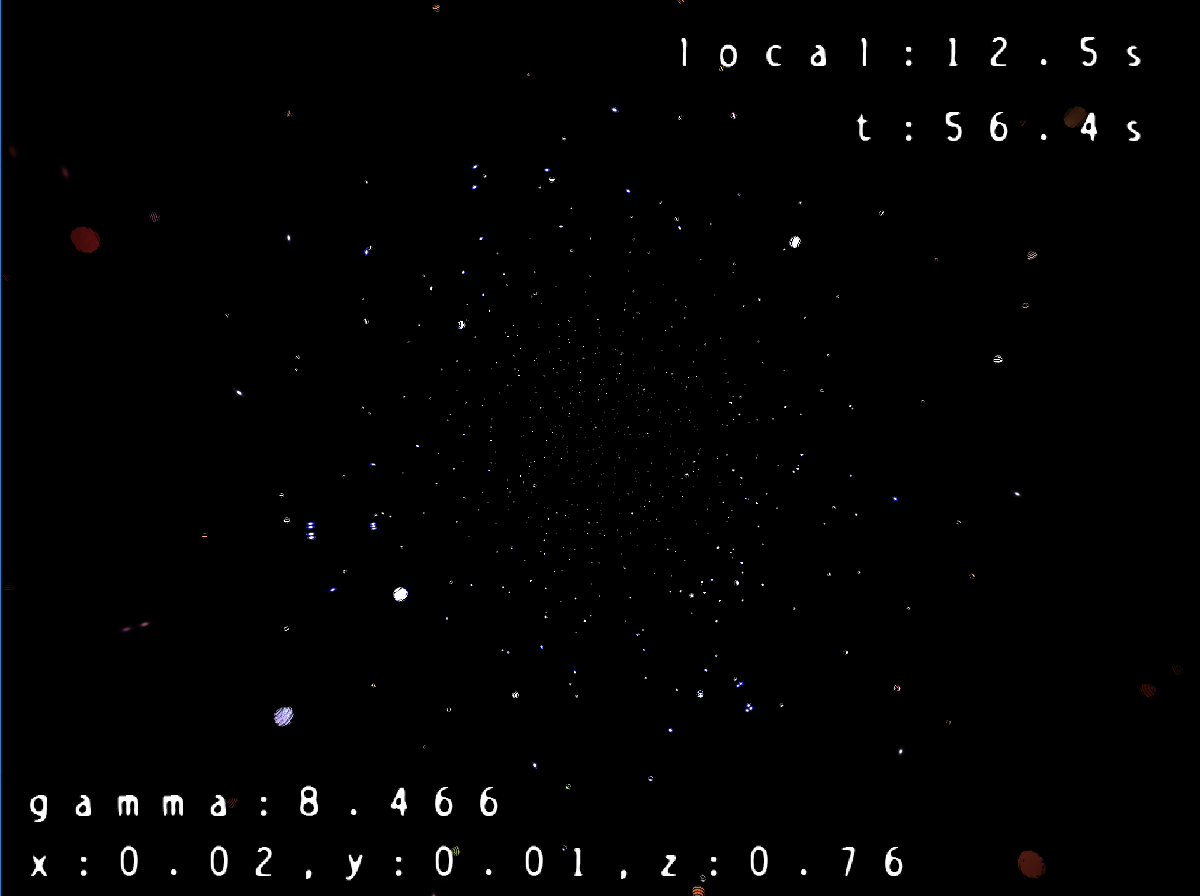
\includegraphics[scale=0.3]{07.png}
	\caption{相对论效果下的前灯效应}
\end{figure}
	
\begin{figure}[H]
\centering
	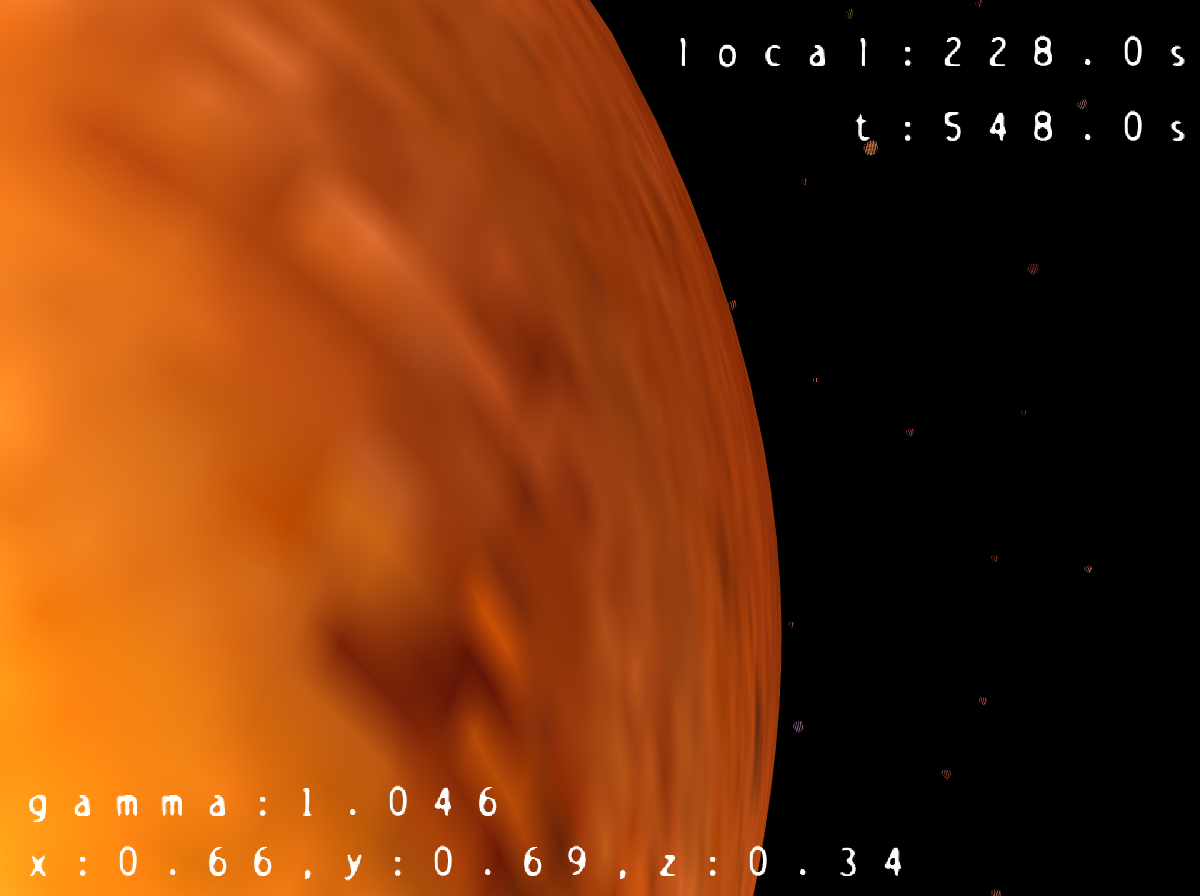
\includegraphics[scale=0.3]{08.png}
	\caption{相对论下的红移效果}
\end{figure}

\subsection{运动和操作}

	飞船在宇宙中会受到恒星的引力作用. 在宇宙中穿行会发现画面抖动, 这是因为不断有恒星在改变恒星的运行轨道. 我们对引力计算的参数值进行了很多修正, 避免飞船的运行轨道发散. 在运行过程中飞船可以最大限度保证能量守恒. (调参由曾嘉熙完成)

\subsubsection{基础操作}

\begin{enumerate}
	\item 前后方向键: 飞船向前/向后加速
	\item 左右方向键: 飞船向左/向右加速,速度过快时将变得无效
	\item WASD: 转动飞船
	\item 鼠标移动: 转动你的头部(相对飞船)
	\item 空格: 将视线变回正对飞船前方
	\item ESC: 退出
\end{enumerate}

\subsubsection{进阶操作}

\begin{enumerate}
	\item Q: 增大引擎功率,有上限
	\item E: 减小引擎功率,有下限
	\item R: 开启相对论视觉效果
	\item T: 关闭相对论视觉效果
\end{enumerate}

\subsubsection{作弊操作}

\begin{enumerate}
	\item 回车: 紧急刹车
	\item P: 暂停/恢复所有行星运动
	\item O: 进入最近的一颗恒星的环绕轨道
\end{enumerate}

\section{分工}

	大作业由秦光辉(1500011398)和曾嘉熙(1500011351)共同完成. 我们工作量相仿(在工作时间的意义下). 具体来说我们完成了程序的不同部分:
	
\begin{itemize}
	\item 程序的框架, 如恒星系统, 行星系统, 贴图纹理资源等由秦光辉完成.
	\item 所有的 GLSL 代码, 包括相对论修正部分, 由曾嘉熙完成.
	\item 随机算法, 密度算法等部分由秦光辉完成.
	\item 运动部分由曾嘉熙完成
	\item Monte Carlo 算法和恒星的在不同距离下的加载由秦光辉完成, 但由曾嘉熙修改完善之后才达到预期效果.
	\item 注释, 文档, Debug 由我们共同合作完成
\end{itemize}

	除一些GL库之外, 我们自己编写的总代码量约 2800 行(包括 GLSL 和 普通 C++ 代码). \\
	
\newpage

\end{CJK*}
\end{document}
